\documentclass[fullpage]{article}
\usepackage{amsmath}
\usepackage{xcolor}
\usepackage{amssymb}
\usepackage{tikz}
\usetikzlibrary{positioning}
\usepackage{amsmath}
\usepackage{amssymb}
\usepackage{color}
\usepackage{tikz}
\usepackage{tikz-cd}
\usepackage{xcolor}
\usetikzlibrary{shapes.geometric}
\usetikzlibrary{backgrounds,fit,decorations.pathreplacing}
\usetikzlibrary{circuits, calc}

\begin{document}

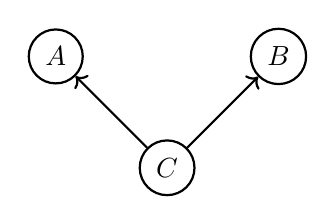
\begin{tikzpicture}[node distance={20mm}, thick, main/.style = {draw, circle}] 
			\node[main] (1) {$C$}; 
			\node[main] (2) [ above left of=1] {$A$}; 
			\node[main] (3) [ above right of=1] {$B$};
			\draw[->] (1) -- (2); 
 			\draw[->] (1) -- (3);
 		\end{tikzpicture}

\end{document}